\section{Na型モンモリロナイトの水和エネルギーモデル}
\subsection{水蒸気の化学ポテンシャル}
粘土含水系が温度$T$,相対湿度$r_H$の水蒸気に接しているとする.
水蒸気は粘土含水系に対して水分浴の役割を果たし,その化学ポテンシャルを$\mu_w$と
すれば,$\mu_w$と$r_H$の関係は次のように表される.
\begin{equation}
	\mu_w
	=
	\mu_w^{sat} +k_BT \log
	\left\{
		\frac{\phi(P_w)}{\phi(P^{sat}_w)}
		r_H
	\right\}
	\label{eqn:mu_rH}
\end{equation}
ただし,$k_B(=1.380649\times 10^{−23}$[J/K]はボルツマン定数,$P_w$と$P^{sat}_w$はそれぞれ 
水分浴の蒸気圧と飽和蒸気圧[Pa]を表す.また,$\phi(P)$は蒸気圧$P$におけるフガシティー係数を表し,
$\mu_w^{sat}$は$P=P^{sat}_w$における水分浴の化学ポテンシャルを意味する.
ここでは,簡単のためフガシティー係数を1にとり,式(\ref{eqn:mu_rH})を
\begin{equation}
	\mu_w
	=
	\mu_w^{sat} +k_BT \log
	\left(
		r_H
	\right)
	\label{eqn:mu_rH_simple}
\end{equation}
として用いる.いま,水分浴kに接して平衡状態にある粘土含水系の化学ポンテンシャルを$\mu$とすれば,
両者の 化学ポテンシャルは一致する.すなわち
\begin{equation}
	\mu=\mu_{w}
	\label{eqn:equiv_mu}
\end{equation}
が成り立つ.
\subsection{粘土含水系の自由エネルギー}
粘土含水系の自由エネルギーを$G$とすれば,系内の水分に関する化学ポテンシャルである$\mu$は,
水分子数$N$の微分
\begin{equation}
	\mu=\frac{\partial G}{\partial N}
	\label{eqn:mu_GN}
\end{equation}
で与えられる.ここで,CG-MD法における自由エネルギーを次のように定義する.
\begin{equation}
	G=\left< \Psi_{LJ} \right> +G_{hyd}
	\label{eqn:Gtot}
\end{equation}
ここで,$\Psi_{LJ}$は粗視化粒子間相互作用に関するポテンシャルエネルギーを,$
G_{hyd}$は層間水の水和に関する自由エネルギーを表す.
$\Psi_{LJ}$はCG-MD法において既に与えられているものだから,
自由エネルギー$G$を定義することと,水和に関する自由エネルギー
$G_{hyd}$を定義することは同義である.
ここでは,平衡状態において式(\ref{eqn:equiv_mu})が満足されるよう
\begin{equation}
	\frac{\partial G}{\partial N}
	=
	\frac{\partial \left< \Psi_{LJ}\right>}{\partial N}
	+
	\frac{\partial G_{hyd}}{\partial N}
	=
	\mu_w^{sat} +k_BT \log
	\left(
		r_H
	\right)
	\label{eqn:equiv_rH}
\end{equation}
から$G_{hyd}$を定める.
以下,$G_{hyd}$を水和エネルギーと呼ぶ.
なお,$\Psi_{LJ}$は,非平衡状態においても
定めることができる.式(\ref{eqn:equiv_rH})は平衡状態において
成り立つ式だから,平衡状態における相互作用ポテンシャルであることを
明示するために$\Psi_{LJ}$でなく$\left< \Psi_{LJ}\right>$と表記している.
非平衡状態を含め,CG-MD系の相互作用ポテンシャルは,
Lenard-Jones対ポテンシャルを
\begin{equation}
	U(\fat{x}_i,\fat{x}_j; \sigma) 
	= 4 \varepsilon 
	\left\{ 
	\left(\frac{\sigma}{r_{ij}}\right)^{12}
	-
	\left(\frac{\sigma}{r_{ij}}\right)^6
	\right\}, \ \ \left( r_{ij}=\left| \fat{x}_i-\fat{x}_j\right| \right)
	\label{eqn:LJ}
\end{equation}
として,
\begin{equation}
	\Psi_{LJ}=\sum_{i<j} U(\fat{x}_i,\fat{x}_j; \sigma) 
	\label{eqn:def_PsiLJ}
\end{equation}
で与えられる.ただし,$\fat{x}_i$と$\fat{x}_j$は,それぞれ第$i$および第$j$番目
の粗視化粒子の位置を表し,
$\varepsilon$は
\begin{equation}
	\varepsilon=1.0\times 10^{-19}, \ \ [{\rm Nm}]
	\label{eqn:eps_of_LJ}
\end{equation}
である.また,パラメータ$\sigma$は,層間距離を制御する変数で,粗視化粒子に水和した水分量としての意味をもつ.
平衡状態における相互作用ポテンシャルは,式\ref{eqn:def_PsiLJ}のアンサンブル平均
\begin{equation}
	\left< \Psi_{LJ}\right>
	=
	\frac{1}{T_d}\int_0^{T_d} \Psi_{LJ}(t)dt
	\label{eqn:Psi_eq}
\end{equation}
で得られる.ただし,
%$M$はCG-MD系における粗視化粒子数,
$T_d$は計算時間,$t$は時間変数を表し,
$\Psi(t)$は時刻$t$におけるポテンシャルエネルギーの瞬間値を意味する.\\

$\<\Psi_LJ >$や$G_{hyd}$は熱力学的なマクロ変数であるから,
温度$T$,圧力$P$, 水分子数$N$を独立変数として表すことができる.
ここでは温度は一定であるとして,$P$と$N$を使い,
\begin{equation}
	G(P,N)=\left< \Psi_{LJ} \right>(P,N) +G_{hyd}(P,N)
	\label{eqn:Gtot_PN}
\end{equation}
と書く.系の体積$V$と化学ポテンシャル$\mu$は,自由エネルギー$G$の微分として
次のように与えられる.
\begin{eqnarray}
	V &= & 
	\left( \frac{\partial G}{\partial P} \right)_N 
	=
	\left( \frac{\partial \left< \Psi_{LJ}\right>}{\partial P} \right)_N 
	+
	\left( \frac{\partial G_{hyd}}{\partial P} \right)_N 
	\label{eqn:G2V}
	\\
	\mu &= & \left( \frac{\partial G}{\partial N} \right)_P 
	=
	\left( \frac{\partial \left< \Psi_{LJ}\right>}{\partial N} \right)_P 
	+
	\left( \frac{\partial G_{hyd}}{\partial N} \right)_P 
	\label{eqn:G2mu}
\end{eqnarray}
ここで,$\left<\Psi_{LJ}\right>$は系の体積と圧力の関係を,
$G_{hyd}$は水分と化学ポテンシャルの関係を定める
自由エネルギー成分となるように,分割されていると仮定する.
すなわち,
\begin{eqnarray}
	\left( \frac{\partial \left< \Psi_{LJ}\right>}{\partial P} \right)_N=0, 
	& \Rightarrow & 
	\left< \Psi_{LJ}\right>(P,N) = \left< \Psi_{LJ}\right>(P) 
	\label{eqn:assuption1}
	\\ 
	\left( \frac{\partial G_{hyd}}{\partial N} \right)_P =0
	& \Rightarrow & 
	\left< G_{hyd}\right>(P,N) = \left< G_{hyd}\right>(N) 
	\label{eqn:G2mu}
	\label{eqn:asumption2}
\end{eqnarray}
のような分割であることを要請する($\Psi_{LJ}$は$N$に依存するが,
$\left<\Psi_{LJ}\right>$をある種の平衡状態について$N$に依存
しないようにすることは可能である).
このとき,式(\ref{eqn:G2mu})は
\begin{equation}
	\mu= \left( \frac{\partial G_{hyd}}{\partial N} \right)_P 
	=
	\frac{dG_{hyd}}{dN}
	\label{eqn:G2mu_2}
\end{equation}
となり,平衡条件(\ref{eqn:equiv_mu})は,
\begin{equation}
	\frac{d G_{hyd}}{d N}
	=
	\mu_w^{sat} +k_BT \log \left( r_H \right)
	\label{eqn:mu_hyd}
\end{equation}
となる.
 従って,式(\ref{eqn:mu_hyd})の両辺を水分子数\(N\)で積分することができれば,
水和エネルギー\(G_{hyd}\)が得られる.しかしながら,
左辺が\(N\)に関する式である一方,右辺は相対湿度\(r_H\)を通じて\(N\)が変数となっている
ため,\(r_H\)と\(N\)の関係を与える必要がある.
%--------------------
\begin{figure}[h]
	\begin{center}
	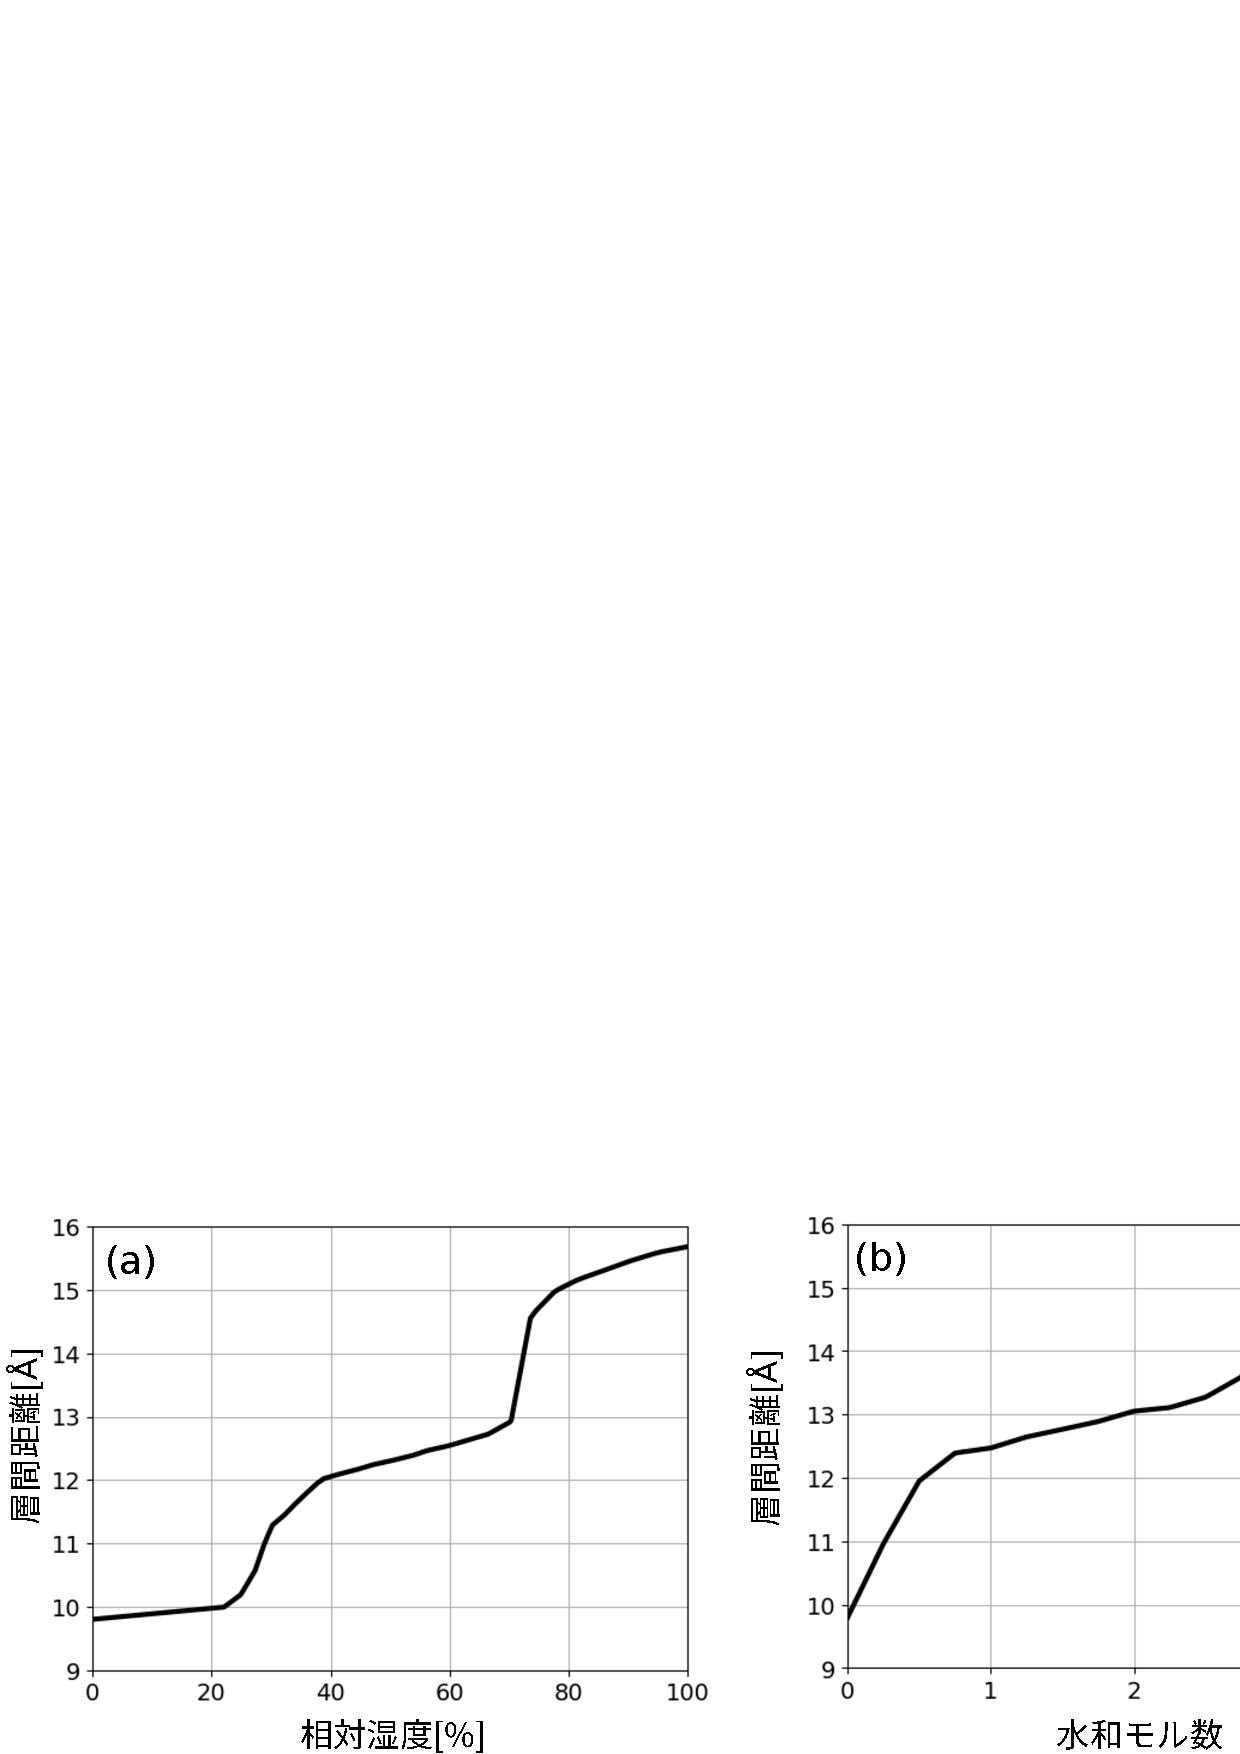
\includegraphics[width=1.0\linewidth]{Figs/fig1.pdf} 
	\end{center}
	\caption{
		Na型モンモリロナイトの膨潤挙動.
		(a) X線回折試験で得られた相対湿度と層間距離の関係(諸留,河村2009\cite{Morodome}
		から再現).(b) 全原子MD計算で得れられた水和モル数と層間距離の関係
		(森本ら2023\cite{Morimoto}). 
	} 
	\label{fig:fig1}
\end{figure}
%--------------------
\begin{figure}[h]
	\begin{center}
	\includegraphics[width=1.0\linewidth]{Figs/fig2.pdf} 
	\end{center}
	\caption{
		Na型モンモリロナイトの膨潤データから作成した
		水和エネルギーモデルと水和モル数の関係.
		(a)化学ポテンシャル$\mu(n)$, (b)水和エネルギーの非線形成分$\delta G_{hyd}(n)$.
	} 
	\label{fig:fig2}
\end{figure}
%--------------------
\subsection{相対湿度と水分子数の関係}
粘土の粉末X線回折試験(X-Ray Diffraction)を行えば,回折ピークから粘土層間の距離
\(h\)が求まる.諸留,河村(2009)は,相対湿度と温度を制御した環境下で
その場X線回折試験を行い,温度一定条件での相対湿度と層間距離の関係
\begin{equation}
	h=h(r_H), \ \ (0 \leq r_H \leq 1)
	\label{eqn:hz_rh}
\end{equation}
を,\(r_H=0\)から1の範囲で詳細に調べている.
%	<img src="FreeEnergy/XRD_swelling.png" width=400, height=300><img>
%	<figcaption>X線回折試験で得られた相対湿度と層間距離の関係</figcaption>
図\ref{fig:fig1}はその結果の一部である,Na型モンモリロナイトに対する
温度50\(^\circ\)Cでの結果を文献から復元したもので,
横軸は相対湿度,縦軸は層間距離を示している.
これを式(\ref{eqn:hz_rh})として用いれば,環境の相対湿度と
粘土含水系の層間距離を結びつけることができる.
従って,層間距離\(h\)と粘土層間の水分子数\(N\)の関係が
得られば,二つの関係式を使って\(r_H\)と\(N\)の関係が与えられ,
式(\ref{eqn:mu_hyd})の両辺を\(N\)あるいは\(r_H\)に変数を
統一して書くことができる.この目的のために,全原子分子動力学法で計算によって
得られた,層間距離と水和モル数\(n\)の関係:
\begin{equation}
	h=h(n)
	\label{eqn:hz_nw}
\end{equation}
を用いる.図\ref{fig:fig1}-(b)は,全原子MD計算から得られた式(\ref{eqn:hz_nw})の
関係で,実験で観測された,相対湿度0から1の間で取り得る
層間距離の範囲でプロットしたものである.
%<figcaption>全原子分子動力学計算で得られた水和モル数\(n\)と層間距離\(h\)の関係</figcaption>
式(\ref{eqn:hz_nw})と式(\ref{eqn:hz_rh})の逆関数\(r_H=r_H(h)\)を合成すれば,
\begin{equation}
	r_H=r_H(h(n))
	\label{eqn:rh_nw}
\end{equation}
が得られ,この関係を計算してグラフ化すると図\ref{fig:fig2}にあるようになる.
%<img src="FreeEnergy/RH_nH2O.png", width=400,height=350><img>
%	<figcaption>
		XRD測定結果の\(h=h(r_H)\)と全原子MD計算結果の\(h=h(n)\)
		から得られた合成関数\(r_H=r_H(n)\).
%</figcaption>
さらに,式(\ref{eqn:rh_nw})を式(\ref{eqn:mu_hyd})に代入し,
\begin{equation}
	N=nN_A, \ \ (N_A=6.023\times 10^{23}:アボガドロ数)
	\label{eqn:}
\end{equation}
であることを考慮すれば,式(\ref{eqn:mu_hyd})の変数を\(n\)に統一した
次の関係が得られる.
\begin{equation}
	\frac{d G_{hyd}}{d n}
	=
	\mu_w^{sat}N_A +k_BN_AT \log \left\{ r_H(n) \right\}
	\label{eqn:mu_hyd_n0}
\end{equation}
ここで,\(\mu_{sat}N_A\)は化学ポテンシャルを1molあたりの
量として表したもので,\(k_B N_A\)は気体定数\(R\)である.
そこで,化学ポテンシャルを[J/mol]の単位で与えるものとして,\(N_A\)を
省略すれば,式\ref{eqn:mu_hyd_n0}は
\begin{equation}
	\frac{d G_{hyd}}{d n}
	=
	\mu_w^{sat} +RT \log \left( r_H(n) \right)
	\label{eqn:mu_hyd_n}
\end{equation}
と表すことができる.これを定温条件で,湿度1を基準として積分すれば,
自由エネルギーの変化
\begin{equation}
	\Delta G_{hyd} = G_{hyd}(n)-G_{hyd}(n_{sat})
	\label{eqn:del_G}
\end{equation}
が
\begin{equation}
	\Delta G_{hyd}
	=
	\mu_{sat}\Delta n
	+
	RT
	\int_{n_{sat}}^{n} \log \left\{ r_H(n)\right\} dn, \ \ (0 \leq n \leq n_{sat})
	\label{eqn:del_G_mu}
\end{equation}
で計算できる.
ただし,\(n_{sat}\)は相対湿度\(r_H=1\)のときに、粉末状の粘土がとる
層間水量で,\(\Delta n\)はその増分
\begin{equation}
	\Delta n = n-n_{sat}
\end{equation}
を意味する. また,粘土含水系の化学ポテンシャルは
\begin{equation}
	\mu
	=
	\frac{d G}{d n}
	\simeq
	\frac{d G_{hyd}}{d n}
	=
	\mu_w^{sat} +RT \log \left\{ r_H(n) \right\}
	\label{eqn:mu_system}
\end{equation}
式(\ref{eqn:mu_system})より,層間水量による化学ポテンシャルの変化は
右辺第二項で与えられ,この項が粘土の膨潤特性を表現している.
また,対応する自由エネルギー変化の成分は,
式(\ref{eqn:del_G_mu})の右辺第二項の積分で与えられる非線形項で,
右辺第1項の\(n\)に関する線形項は,粘土の膨潤特性とは関係しない.
そこで,
\begin{equation}
	\delta \mu = \mu-\mu_{w}^{sat}
	=
	RT \log \left\{ r_H(n)\right\} dn
\end{equation}
\begin{equation}
	\delta G_{hyd} =
	RT
	\int_{n_{sat}}^{n} \log \left\{ r_H(n)\right\} dn
\end{equation}
として,これらの\(n\)に対する変化を描くと,下の図に示す結果が得られる.
% <img src="FreeEnergy/Muvar_nH2O.png", width=400, height=350></img>
%<figcaption> 水和モル数と化学ポテンシャルの湿度依存項\(\delta \mu\)の関係 </figcaption>
%
%<img src="FreeEnergy/Gvar_nH2O.png", width=400, height=350></img>
%<figcaption> 水和モル数と水和自由エネルギーの湿度依存項\(\delta G_{hyd}\)の関係 </figcaption>
%--------------------
\subsection{粒子間相互作用力}
CGMD法では,粗視化粒子に作用する力として分子内力と分子間力の2つを与える.
分子内力は,粗視化粒子を結合して一つの分子として振る舞うように剛性を与える
もので,本CGMD法では同一分子内で隣接する粗視化粒子を線形バネで結合すること
によって与えている.そのため,無応力状態では一つの分子を表現する粗視化粒子群
は直線上に整列する.
分子間力はファンデルワールス力の基本的なモデルであるレナード-ジョーンズ対ポテンシャル
(以下LJポテンシャル呼ぶ):
\begin{equation}
	U(\fat{x}_i,\fat{x}_j; \sigma) 
	= 4 \varepsilon 
	\left\{ 
	\left(\frac{\sigma}{r_{ij}}\right)^{12}
	-
	\left(\frac{\sigma}{r_{ij}}\right)^6
	\right\}, \ \ \left( r_{ij}=\left| \fat{x}_i-\fat{x}_j\right| \right)
	\label{eqn:LJ}
\end{equation}
で与える.

LJポテンシャルは粒子間距離$r_{ij}$が小さいときに斥力を,大きいときに引力を粒子間に作用させる.
引力と斥力は概ね$r_{ij}=1.1\sigma$を境に切り替わる.
斥力が作用する領域では$r_{ij}\rightarrow 0$に向けて斥力が急増する.
従って,$r_{ij}=\sigma$は粗視化粒子の接近限界とみなすことができる.
水を非圧縮性物質とみなせば,粗視化粒子の接近限界は粘土分子が当該位置でもつ
水和水量で決まる.いま,粒子$i$のもつ水和層の厚みが$s_i$,
粒子$j$のそれが$s_j$であったとする.無水状態での粘土分子層の厚さを$\sigma_0$とすれば,
粗視化粒子の接近限界$\sigma$は次の式で与えられる.
\begin{equation}
	\sigma=\sigma_0 +s_i+s_j
	\label{eqn:}
\end{equation}
このことより,粗視化粒子の有する水和水層の厚さ$s_i$を定めればLJポテンシャルの
特性距離$\sigma$が決まり,水和水の量や分布に応じた粒子間相互作用を与えることができる.
CGMD法では,各粗視化粒子は位置$\fat{x}$と速度$\fat{v}$,向き$\fat{n}$を属性として持つ.
ここで,粘土分子の一方の面を正方向$\fat{n}$とし,その反対の方向を$-\fat{n}$とすれば,
これら2つの方向それぞれに水和水が存在するため,$\pm\fat{n}$方向の水和水層厚を
区別する場合$s^\pm$, 文脈から明らかな場合は$\pm$を省略して$s_i$などと書く.
ここに,$i$は粗視化粒子番号を意味する.粒子番号についても明示する必要の無い場合は省略し
単に$s$と書く.これら$\fat{x},\fat{v},\fat{n}$および$s$は全て未知量である.
これらのうち$\fat{x}$と$\fat{v}$は,運動方程式:
\begin{equation}
	m\dot{ \fat{v}}=\fat{F}_K+\fat{F}_{LJ}, \ \ \fat{v}=\dot{\fat{x}}
	\label{eqn:eq_motion}
\end{equation}
を時間積分することで与えられた初期状態から繰り返し状態を更新する.
なお,$m$は粗視化粒子の質量を, $\fat{F}_K$と$\fat{F}_{LJ}$は,
それぞれ分子内および分子間力を表す.粒子の向き$\fat{n}$は,分子を構成する
粗視化粒子の位置座標から各粒子位置での接ベクトルを求め,それに直交する方向として定める.
水和水層の厚さ$s$は,後に述べるように水和エネルギーと粒子間相互作用エネルギー
の停留条件から決定する.水和水層の厚さ$s$とX線回折試験から求められている
膨潤状態および層間距離は表\ref{tbl:tbl_sig}の通りである.
\begin{table}[h]
	\begin{center}
	\caption{分子間相互作用ポテンシャルにおける特性距離と膨潤状態の対応.}
	\vspace{3mm}
	\begin{tabular}{c||c|c|c|c|c}
		膨潤状態 & 0層 & 1層 & 2層 & 3層 & $\cdots$\\
		\hline
		特性距離(層間距離)$\sigma$[{\rm nm}]& 0.9 & 1.2 & 1.5 & 1.8 & $\cdots$ \\
		\hline
		水和水層厚$s$[{\rm nm}] & 0.0 & 0.15 & 0.30 & 0.45 & $\cdots$
	\end{tabular}
	\label{tbl:tbl_sig}
	\end{center}
\end{table}
%--------------------
\subsubsection{振動モデル}
X線回折試験の結果から,Na型モンモリロナイトは相対湿度の増加に対して階段状に
層間距離を変化させることが知られている.層間距離は,概ね水分子整数個分程度となり,
水分子$n$個相当の層間距離にある状態を$n$層膨潤と呼ぶ.
Na型モンモリロナイトは0層膨潤から1層,2層膨潤と推移し,例えば1.5層といった
中間的な膨潤状態を取ることは少ない.このような挙動は水和エネルギー関数に
単調モデルを用いた場合に生じ得ない.これは,整数次の膨潤状態に相当する
水和水層厚で,水和エネルギー関数が何ら特別な特徴を持たないためである.
そこで,水分子サイズに相当する周期で変化する振動成分を単調モデルに加えた
水和エネルギーモデルを用いることで,どのように膨潤挙動の違いが現れるかを調べる.

$n$層($n=1,2,\dots$)膨潤状態における水和水層の厚さ$s$は,
表\ref{tbl:tbl_sig}に示すように,0.15nmの倍数である.
そこで,周期0.15nmの振動成分を単調モデルに加えることを考える.
図\ref{fig:fig2}(a)に,黒の実線でこの方法で作成した振動成分を有する
水和エネルギーモデルを示す.以下,この水和エネルギーモデルを振動モデルと呼ぶ.
%--------------------
